\documentclass[12pt,a4paper,oneside]{report}

% --- Jazyková a typografická nastavení (Language & Typography) ---
\usepackage[utf8]{inputenc}
\usepackage[czech]{babel}
\usepackage[T1]{fontenc}
\renewcommand{\familydefault}{\sfdefault}

% --- Geometrie stránky a řádkování (Page Geometry & Spacing) ---
\usepackage{geometry}
\geometry{
    a4paper,
    top=25mm,
    bottom=25mm,
    left=30mm,   % Větší prostor pro případnou vazbu
    right=25mm
}
\usepackage{setspace}

% --- Balíčky pro matematiku a grafiku (Math & Graphics) ---
\usepackage{amsmath}
\usepackage{amsfonts}
\usepackage{amssymb}
\usepackage{graphicx}
\usepackage{newunicodechar}
\newunicodechar{−}{-}
\usepackage{xcolor}

% --- Nastavení zdrojových kódů (Source Code Setup) ---
\usepackage{listings} % Odstraněn parametr [listof], který způsoboval reset do angličtiny
\renewcommand{\lstlistingname}{Zdrojový kód}

\makeatletter
\renewcommand\lstlistoflistings{%
    \chapter*{Seznam zdrojových kódů}% Přímé vynucení českého názvu o velikosti kapitoly
    \addcontentsline{toc}{chapter}{Seznam zdrojových kódů}% Volitelné: přidá seznam i do Obsahu
    \@starttoc{lol}% Načtení obsahu souboru .lol
}
\makeatother

% Definice vzhledu pro ukázky kódů (např. Rust/TypeScript)
\lstset{
    backgroundcolor=\color{gray!5},
    basicstyle=\ttfamily\small,
    breakatwhitespace=false,         
    breaklines=true,                 
    captionpos=b,                    
    commentstyle=\color{green!50!black},
    keywordstyle=\color{blue},
    stringstyle=\color{orange},
    frame=single,
    numbers=left,
    numberstyle=\tiny\color{gray},
    rulecolor=\color{black!30},
    tabsize=4,
    showstringspaces=false
}

% --- Křížové odkazy a hyperodkazy (Hyperlinks) ---
\usepackage[unicode]{hyperref}
\hypersetup{
    colorlinks=true,
    linkcolor=black,      % Pro tiskovou verzi je lepší nechat černé, 
    citecolor=blue,       % nebo změnit na barvy, pokud odevzdáváš pouze PDF
    urlcolor=teal
}

% --- bib
\usepackage[autostyle=true,czech=quotes]{csquotes} % Správné uvozovky
\usepackage[backend=biber, style=iso-numeric, alldates=iso]{biblatex} % Bibliografie dle ISO 690
\addbibresource{literature.bib} % Import souboru s literaturou

% --- acronyms
\usepackage{acronym}

% --- Metadata Dokumentu ---
\title{
    {\Huge\bfseries Klasifikace astronomických fotografií}\\[0.4cm]
    {\LARGE Semestrální projekt}\\[1.5cm]
}
\author{\large\bfseries Patrik Mintěl}
\date{\large \today}

% =========================================================================
% INDIVIDUAL CHAPTER TEXTS (In Czech as requested)
% =========================================================================
\begin{document}

% --- Titulní strana ---
\maketitle

% --- Nečíslované povinné seznamy ---
\pagenumbering{roman}

\tableofcontents
\cleardoublepage

% --- Seznam zkratek ---
\include{acronyms}

\clearpage
\listoffigures

%\clearpage
%\lstlistoflistings

\listoftables
\clearpage

% --- Reset číslování pro hlavní obsah ---
\cleardoublepage
\pagenumbering{arabic}

% =========================================================================
% HLAVNÍ KAPITOLY DOKUMENTU
% =========================================================================

\chapter{Úvod}
\label{ch:introduction}

Digitální astrofotografie hlubokého vesmíru prošla v posledním desetiletí masivním technologickým vývojem, především díky přechodu od klasických \ac{CCD} snímačů k vysoce citlivým \ac{CMOS} architekturám. Tento posun umožnil zachycovat rozsáhlé struktury s vysokým kvantovým ziskem, avšak přinesl s sebou kritickou výzvu v podobě exponenciálního nárůstu objemu generovaných dat. Výsledná kvalita finálního obrazu je přímo závislá na statistickém sloučení desítek až stovek dílčích expozic. Během několikahodinových akvizičních sekvencí však dochází k neustálým změnám atmosférických podmínek, poryvům větru, chybám v mechanickém vedení montáže nebo k přechodům oblačnosti a umělých družic. Všechny tyto jevy vnášejí do datové sady anomálie a deformace hvězdných profilů.

Tradiční lidská kontrola a manuální vyřazování poškozených snímků (tzv. \textit{culling}) představuje v moderní astrofotografické praxi časově náročné a vysoce subjektivní úzké hrdlo. Předložená práce se proto zabývá návrhem, architekturou a implementací desktopového systému, který tento proces plně automatizuje na základě exaktních statistických a fyzikálních parametrů bodových zdrojů.

Obsah této práce je strukturován do sedmi navazujících kapitol:
\begin{itemize}
    \item \textbf{Kapitola 2} se věnuje hluboké analýze astronomického souborového formátu \acs{FITS}, popisu jeho vnitřní datové struktury a algoritmickému návrhu pro metadatový \textit{fingerprinting}, který slouží k bezpečné automatické segmentaci kalibračních relací.
    \item \textbf{Kapitola 3} rozebírá matematicko-fyzikální základy profilování hvězd. Zaměřuje se na komparaci robustnosti metrik \acs{FWHM} a \acs{HFR}, výpočet excentricity profilů pomocí prostorových momentů druhého řádu a mřížkovou estimaci pozadí.
    \item \textbf{Kapitola 4} popisuje výpočetní zpracování signálu a pixelovou aritmetiku redukce systematických chyb, včetně streamovaných streamingových výpočtů statistických předloh (\textit{Master} snímků).
    \item \textbf{Kapitola 5} se zaměřuje na softwarovou architekturu celého systému, kde je rozebráno propojení reaktivního webového frontendu s vysoce výkonným nativním jádrem a paralelním modelem konkurence.
    \item \textbf{Kapitola 6} se zabývá nelineárními transformacemi dynamicého rozsahu surových dat pro účely lidské vizualizace a popisuje hardwarovou akceleraci vykreslovacího enginu.
    \item \textbf{Kapitola 7} detailně specifikuje samotnou implementační logiku dvouprůchodového skórování, uživatelské řízení prahových hodnot a deterministické ochranné pojistky hodnotícího systému.
    \item \textbf{Kapitola 8} v závěru přináší výkonnostní a kritickou analýzu celého řešení nad reálným komplexním datasetem a definuje roadmapu přechodu k modelům hlubokého učení v navazující diplomové práci.
\end{itemize}
\chapter{Astronomické datové formáty a zpracování metadat}
\label{ch:formats}
\section{Struktura souboru FITS} \label{sec:fits_structure}
Formát \textbf{\ac{FITS}} je nejpoužívanější datový formát v astronomii pro přenos, analýzu a archivaci vědeckých datových sad. Není to pouze jednoduchý obrazový formát (jako například JPG nebo GIF), ale je primárně navržen tak, aby dokázal ukládat komplexní vědecká data skládající se z vícerozměrných polí (obrazů) a dvourozměrných tabulek organizovaných do řádků a sloupců. 
\subsection{Základní uspořádání a HDU} Základním stavebním kamenem souboru \ac{FITS} je tzv. \textbf{\ac{HDU}}. Každý \ac{FITS} soubor se skládá z jednoho nebo více těchto segmentů. První \ac{HDU} v souboru je povinné a nazývá se \textbf{primární HDU} (Primary HDU).
\ac{FITS} soubor obsahující pouze primární HDU je označován jako \textit{Single Image FITS} (SIF) nebo \textit{Basic FITS}. Za primárním \ac{HDU} však může následovat libovolný počet dalších \ac{HDU}, které se nazývají \textbf{rozšíření} (extensions). Takové soubory se označují jako \textit{Multi-Extension FITS} (MEF).
Fyzická i logická struktura celého souboru je přísně formátována do \textbf{logických bloků (záznamů) o přesné velikosti 2880 bajtů} (odpovídá 23040 bitům). Každé \ac{HDU} se skládá z hlavičky (Header Unit) a datové části (Data Unit), přičemž každá z těchto částí je zarovnána na násobky 2880 bajtů. Pokud data nebo hlavička tento blok zcela nevyplní, je zbytek bloku doplněn mezerami ve formátu ASCII (v hlavičce) nebo nulovými bity (v datové části).\cite{fits_standard}
\subsection{Hlavička (Header Unit)} Hlavička každého \ac{HDU} obsahuje metadata o datech a skládá se z formátovaného ASCII textu. Je tvořena sekvencí \textbf{80znakových textových řetězců} (card images), z nichž každý obvykle definuje jeden klíč ve formátu: \begin{verbatim} KLÍČ    = hodnota / volitelný komentář \end{verbatim} Název klíče (keyword name) smí obsahovat maximálně 8 znaků a je omezen pouze na velká písmena anglické abecedy, číslice, spojovník a podtržítko.
Každá hlavička začíná sekvencí povinných klíčů v přesně daném pořadí. Pro primární hlavičku to jsou: \begin{itemize} \item \textbf{SIMPLE}: Logická hodnota (T/F) udávající, zda soubor plně vyhovuje standardu \ac{FITS}. \item \textbf{BITPIX}: Celočíselná hodnota určující počet bitů na jeden datový prvek (pixel). Platné hodnoty jsou 8, 16, 32 pro celá čísla a -32 nebo -64 pro čísla s plovoucí řádovou čárkou podle standardu IEEE. \item \textbf{NAXIS}: Počet os v přidruženém datovém poli (hodnota 0-999). Hodnota 0 znamená, že po hlavičce nenásledují žádná obrazová data. \item \textbf{NAXISn}: Sériový klíč (např. NAXIS1, NAXIS2) definující velikost podél každé příslušné osy n. \end{itemize} Na samotný konec metadat v rámci hlavičky je vždy vyžadován klíč \textbf{END}, po kterém je zbytek 2880bajtového bloku hlavičky doplněn mezerami.\cite{fits_standard}
\subsection{Datová část (Data Unit)} Datová část, pokud je definována (při \texttt{NAXIS > 0}), bezprostředně následuje za posledním blokem hlavičky. V případě obrazových dat je pole pixelů uloženo jako souvislý proud bitů bez mezer či výplňových znaků uprostřed. U vícerozměrných polí se data ukládají sekvenčně tak, že index podél první osy (\texttt{NAXIS1}) se mění nejrychleji, a u dalších os se mění postupně pomaleji, což je konvence převzatá z programovacího jazyka Fortran.
Nativně \ac{FITS} nepodporuje datový typ neznaménkových celých čísel (unsigned integer) větších než 8 bitů. Řeší to však obecně uznávanou konvencí, podle které se hodnoty ukládají jako znaménková čísla (signed) s aplikací fixního offsetu. Offset se z definice ukládá pomocí hlavičkového klíče \texttt{BZERO} (často v kombinaci s koeficientem \texttt{BSCALE}).\cite{fits_standard}
\subsection{Standardní rozšíření (Extensions)} Současný standard \ac{FITS} plně specifikuje tři základní typy rozšíření (extensions), které umožňují ukládat komplexní datové struktury do jediného souboru: \begin{enumerate} \item \textbf{Image Extensions} (\texttt{XTENSION = 'IMAGE'}): Obsahují vícerozměrné pole pixelů stejným způsobem jako primární \ac{HDU}. \item \textbf{ASCII Table Extensions} (\texttt{XTENSION = 'TABLE'}): Ukládají tabulková data organizovaná do řádků a sloupců, přičemž všechny číselné i textové položky jsou kódovány ve formátu ASCII. Jsou snadněji čitelná pro lidi, avšak výpočetně a paměťově méně efektivní. \item \textbf{Binary Table Extensions} (\texttt{XTENSION = 'BINTABLE'}): Ukládají tabulková data v binární reprezentaci, což zajišťuje kompaktnější velikost a rychlejší zpracování dat (čtení i zápis) ve srovnání s ASCII tabulkami. Binární tabulky jsou vysoce flexibilní a v každé buňce pole umožňují uložení celého vícerozměrného pole pomocí konvencí pro pole s proměnnou délkou (Variable Length Arrays), která jsou odkazována formou tzv. heap oblasti uvnitř datové části. \end{enumerate}
\begin{figure}[htbp] 
    \centering 
    \begin{verbatim} 
        +===================================================+ 
        |                   Primární HDU                    | 
        |---------------------------------------------------| 
        | Primární hlavička (Header Unit)                   | 
        | (bloky 2880 bajtů, klíče SIMPLE, BITPIX, atd.)    | 
        |---------------------------------------------------| 
        | Primární data (Data Unit) - volitelná             | 
        | (bloky 2880 bajtů, vícerozměrné pole bitů)        | 
        +===================================================+ 
        |                 HDU Rozšíření 1                   | 
        |---------------------------------------------------| 
        | Hlavička rozšíření (XTENSION='IMAGE'|'BINTABLE')  | 
        | (bloky 2880 bajtů)                                | 
        |---------------------------------------------------| 
        | Data rozšíření (Data Unit) - volitelná            | 
        | (bloky 2880 bajtů)                                | 
        +===================================================+ 
        |                 HDU Rozšíření N                   | 
        |                      ...                          | 
        +===================================================+ 
    \end{verbatim} 
    \caption{Schéma blokové struktury souboru ve formátu FITS.} 
    \label{fig:fits_structure} 
\end{figure}
\section{Metadatový fingerprinting a segmentace relací}
Tato kapitola popisuje dvoufázový proces kategorizace a třídění souborů ve formátu \textbf{\ac{FITS}}. Pro správnou kalibraci a zpracování astrofotografických dat je nezbytné snímky rozdělit do logických celků (relací) a ke světelným snímkům (light frames) správně přiřadit odpovídající kalibrační data. Proces se skládá ze základní textové segmentace na základě adresářové struktury a z pokročilého seskupování pomocí extrakce metadat.
\subsection{Segmentace pomocí prefixů a sufixů v cestě k souboru}
Prvním krokem, který se provádí ihned po importu souborů skrze uživatelské rozhraní (\textbf{\acs{UI}}), je rozdělení na základě uživatelsky definované adresářové struktury. Uživatel si v aplikaci může definovat množinu prefixů nebo sufixů, podle kterých se analyzuje absolutní cesta k souboru.
Uvažujme například následující strukturu složek a souborů: 
\begin{verbatim} 
FILES/Object {OBJECT}/Session {YYYY-MM-dd}/{LIGHT/DARK/FLAT/BIAS}/*.fits 
\end{verbatim}
Konkrétní plná cesta k souboru pak může vypadat následovně: \texttt{FILES/Object M31/Session 2026-02-01/2026-02-01-00-05-13--20.00-LIGHT-NOFILTER.fits}.
Při vložení souborů se aplikují definované rozdělovače (např. prefixy \texttt{"Object "} a \texttt{"Session "}) které si uživatel nastavuje v nastavení viz Obrázek \ref{fig:prefix_suffix_settings}. 

\begin{figure}[h] 
    \centering 
    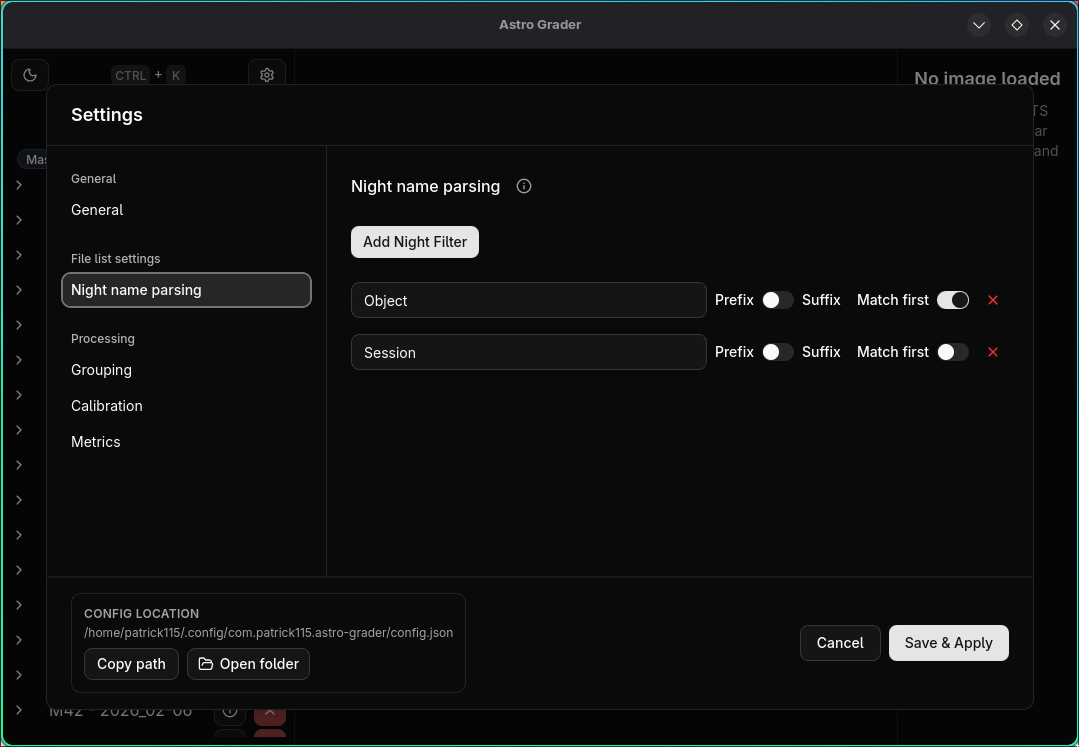
\includegraphics[width=0.8\textwidth]{assets/parsing_settings.png} 
    \caption{Ukázka nastavení prefixů a sufixů v \acs{UI} pro analýzu adresářové struktury.} 
    \label{fig:prefix_suffix_settings} 
\end{figure}

Výsledkem tohoto prvotního průchodu je logické roztřídění souborů do konkrétních pozorovacích nocí a objektů (například \texttt{M31 - 2026-02-01} nebo \texttt{Orion M42 - 2025-12-24}) viz Obrázek \ref{fig:showcase_nights}. Všechny soubory náležející dané noci a objektu jsou v rámci \acs{UI} umístěny společně. Soubory, které nevyhovují žádnému z definovaných pravidel, jsou přesunuty do kategorie \textit{Nezařazeno} (Unsorted).

\begin{figure}[h] 
    \centering 
    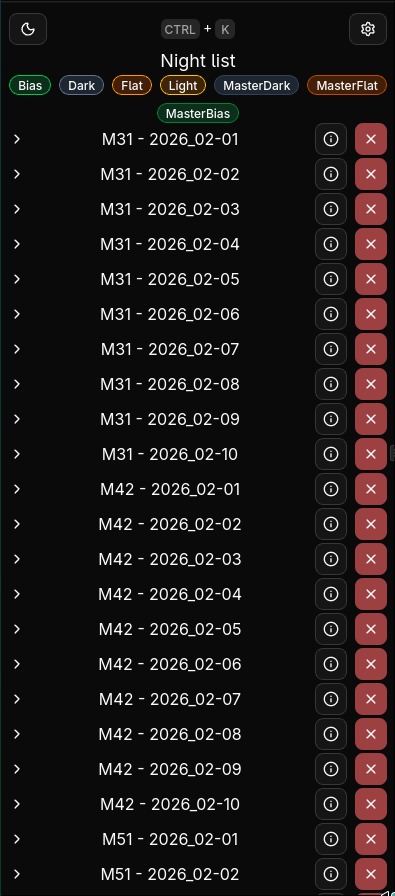
\includegraphics[width=0.4\textwidth]{assets/night_list.png} 
    \caption{Zobrazení rozdělených pozorovacích nocí a objektů po prvotním importu.} 
    \label{fig:showcase_nights} 
\end{figure}

\subsection{Seskupování a metadatový fingerprinting (Grouping)} Druhým, pokročilejším krokem je tzv. proces \textit{Grouping} (seskupování). V této fázi se analyzuje fyzický obsah hlaviček souborů \ac{FITS}, kde se čtou základní hodnoty z \ac{FITS} klíčů a tagů. Z každého snímku je tak vytvořen metadatový \uv{otisk} (tzv. fingerprint), který typicky obsahuje parametry jako: 
\begin{itemize} 
    \item \textbf{Zdrojová noc} (Source night) - odvozena z prvního kroku na základě adresářové struktury, např. M31 - 2026-02-01. 
    \item \textbf{Kamera} (Camera) - identifikována z klíčů \texttt{INSTRUME}, \texttt{CCDNAME} nebo \texttt{CAMERA}. 
    \item \textbf{Filtr} (Filter) - určující použitý optický filtr z klíče \texttt{FILTER}. 
    \item \textbf{Teleskop} (Telescope) - identifikátor optické soustavy čtený z klíčů \texttt{TELESCOP} nebo \texttt{FOCALLEN}. 
    \item \textbf{Délka expozice} (Exposure time) - hodnota expozičního času získána z klíčů \texttt{EXPTIME} nebo \texttt{EXPOSURE}. 
    \item \textbf{Zisk senzoru} (Gain) - hodnota elektronického zesílení načtena z klíčů \texttt{GAIN} nebo \texttt{EGAIN}. 
    \item \textbf{Teplota senzoru} (Temperature) - aktuální či cílová teplota čipu z klíčů \texttt{CCD-TEMP} nebo \texttt{SET-TEMP}. 
\end{itemize} 
Na základě těchto otisků a logiky definované ve zdrojových kódech aplikace se následně tvoří dedikované metadatové koše (Session Buckets), do kterých se snímky automaticky skládají.
Základem každé takové vytvořené skupiny jsou vždy \textbf{světelné snímky} (Light frames), které zůstávají zachovány ve svém zařazení do konkrétní noci z prvního kroku. K těmto světelným datům jsou následně z celého datasetu (včetně složky \textit{Nezařazeno}) algoritmicky vyhledána a přiřazena odpovídající kalibrační data: 
\begin{enumerate} 
    \item \textbf{Temné snímky (Dark frames):} Algoritmus nejprve zjišťuje, zda existuje pro danou skupinu odpovídající \textit{Master Dark} — tedy referenční snímek vzniklý statistickou integrací mnoha samostatných temných expozic, který slouží k odstranění tepelného šumu. Pokud ano, přiřadí se. V opačném případě se z noci nebo z nezařazené složky vyberou všechny jednotlivé \textit{Dark} snímky, jejichž metadata (jako expozice, zisk a teplota) korespondují se světelnými snímky dané skupiny. 
    \item \textbf{Snímky plochého pole (Flat frames):} Proces je obdobný jako u temných snímků. Upřednostňuje se případný \textit{Master Flat} — kalibrační snímek vytvořený sloučením dílčích snímků, který mapuje optické vady jako je vinětace či stíny prachových částic. Jinak se vyhledávají běžné \textit{Flat} snímky podle shody metadat (zejména zisku, případně použitého filtru a teleskopu). 
    \item \textbf{Ofsetové snímky (Bias frames):} Shodně se aplikuje logika vyhledávání \textit{Master Bias} — což je referenční obraz vzniklý složením snímků s nulovou expoziční dobou, izolující konstantní elektronický šum vygenerovaný procesem čtení dat ze senzoru — nebo běžných \textit{Bias} snímků s vyhovujícím ziskem a charakteristikou kamery. 
\end{enumerate}
Tento exaktní přístup zajišťuje, že se k dané sadě světelných snímků neomylně přiřadí pouze taková kalibrační data, která byla pořízena za odpovídajících hardwarových a teplotních podmínek, čímž je zaručen bezchybný průběh následné kalibrace.
\begin{figure}[htbp] 
    \centering 
    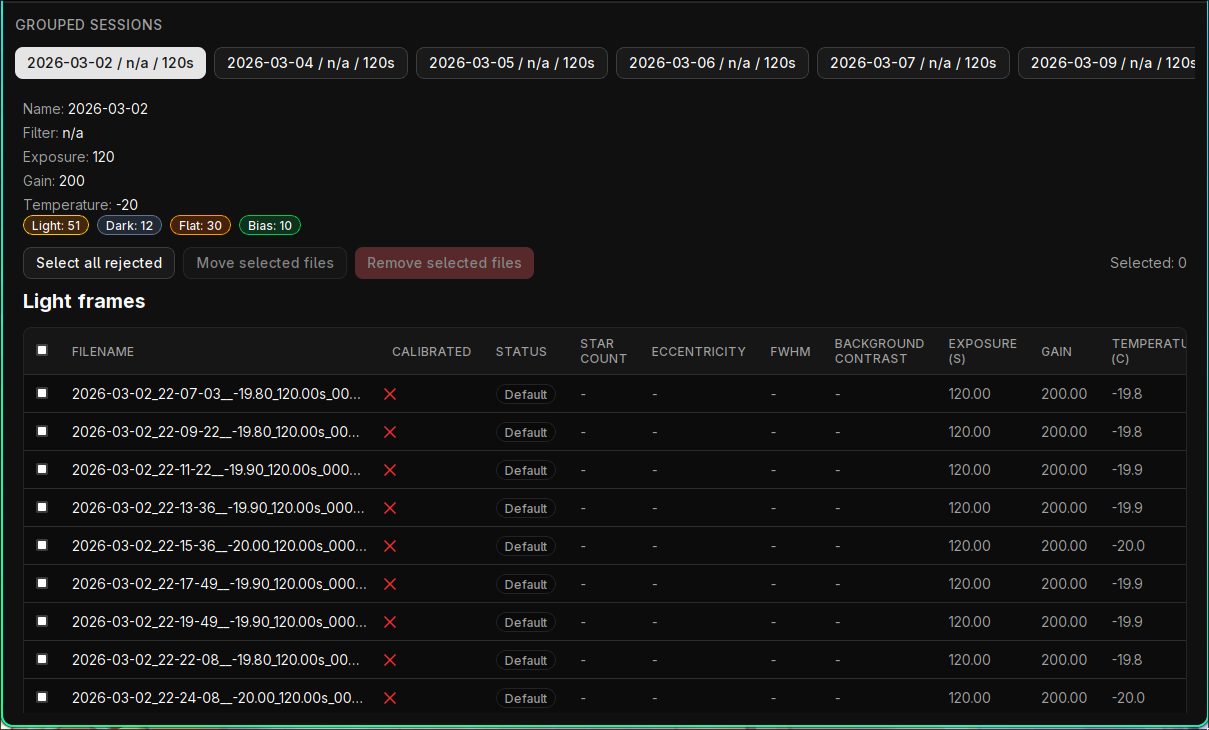
\includegraphics[width=0.8\textwidth]{assets/grouped_nights.png}
    \caption{Ukázka finálně sestavených skupin (Groups) obsahujících světelné snímky a k nim matematicky spárovaná kalibrační data na základě metadatového fingerprintingu.} 
    \label{fig:showcase_groups} 
\end{figure}
\chapter{Matematická fyzika extrakce zdrojů a profilování hvězd}
\label{ch:math}

Tato kapitola stručně popisuje základní matematické a fyzikální principy, pomocí kterých analyzujeme tvar hvězd a vlastnosti pozadí na astronomických snímcích. Abychom dokázali spolehlivě zhodnotit kvalitu pořízené expozice, musíme vzít surová data z kamery – tedy obyčejnou mřížku pixelů nesoucí číselné hodnoty jasu – a matematicky je přepočítat na skutečné fyzikální vlastnosti vyfocených objektů. Zjišťujeme z nich tak například \textbf{celkové množství světla (flux) a přesnou velikost nebo tvar hvězdy} oddělené od rušivého jasu pozadí

\section{Profilování bodových zdrojů (FWHM vs. HFR)}
Kvantifikace průměru hvězd slouží jako primární indikátor zaostření a okamžitého stavu atmosférického neklidu (\textit{seeing}). Distribuce jasu bodového zdroje je v ploše snímače popsaná funkcí rozptylu bodu — \ac{PSF}. Tradičně se pro tento účel využívá aproximace Gaussovou funkcí a měření metriky \ac{FWHM}, která udává šířku profilu v polovině jeho maximální intenzity. Pro ideální izotropní distribuci platí vztah:
\begin{equation}
\text{FWHM} \approx 2.35482 \cdot \sigma
\end{equation}
kde $\sigma$ reprezentuje směrodatnou odchylku rozdělení jasu. Výpočetní jádro systému využívá pro odhad \ac{FWHM} adaptivní modifikaci, pracující s délkami poloos $a$ a $b$, získanými z prostorových momentů obrazu \cite{sextractor}: $\text{FWHM} = 2.3548203 \cdot \sqrt{a \cdot b}$.

Tento matematický model však vykazuje závažné limity při silném rozostření. U zrcadlových dalekohledů dochází vlivem centrálního stínění sekundárním zrcadlem k deformaci \ac{PSF} do tvaru mezikruží (toroidu). Gaussovo prokládání v takovém případě selhává, algoritmus nedokáže spolehlivě lokalizovat vrchol amplitudy a vypočtená hodnota \ac{FWHM} ztrácí stabilitu.

Z tohoto důvodu se jako robustnější klasifikační alternativa zavádí poloměr polovičního toku energie — \ac{HFR} (respektive průměr \ac{HFD}, kde platí $\text{HFD} = 2 \cdot \text{HFR}$). Tato integrální metrika definuje poloměr kruhové apertury kolem těžiště hvězdy, uvnitř které se nachází přesně polovina celkového emitovaného světelného toku $F_{\text{total}}$ \cite{hfr}:
\begin{equation}
\int_{0}^{R_{\text{HFR}}} 2\pi r \cdot [I(r) - I_{\text{bg}}] \, dr = \frac{1}{2} F_{\text{total}}
\end{equation}

Protože \ac{HFR} integruje energii z celé plochy objektu, vykazuje vysokou odolnost vůči vysokofrekvenčnímu šumu a lineárně škáluje i u prstencových profilů rozostřených hvězd. V systému se proto \ac{HFR} využívá ke sledování stability zaostření napříč nocí, zatímco \ac{FWHM} slouží jako doplňkový indikátor pro detekci směrového rozmazání snímku.

\section{Centrální momenty obrazu a výpočet excentricity}
Excentricita popisuje míru eliptického protažení hvězd a indikuje mechanické či atmosférické poruchy, jako jsou chyby pointace montáže, průhyby tubusu nebo poryvy větru. Výpočet tvarových parametrů bodových zdrojů vychází z teorie prostorových momentů diskrétní distribuce intenzit $I(x, y)$ řádu $(p+q)$ \cite{popowicz}:
\begin{equation}
M_{pq} = \sum_{x} \sum_{y} x^p y^q \cdot I(x, y)
\end{equation}

Z momentů nultého a prvního řádu se určují souřadnice těžiště objektu $(\bar{x}, \bar{y})$. Pro zajištění invariance vůči posunutí v ploše snímače se následně počítají centrální momenty druhého řádu $\mu_{pq}$, ze kterých se konstruuje symetrická matice kovariance:
\begin{equation}
\mathbf{\Sigma} = \frac{1}{M_{00}} \begin{pmatrix} \mu_{20} & \mu_{11} \\ \mu_{11} & \mu_{02} \end{pmatrix}
\end{equation}

Analytickým řešením této matice (nalezením vlastních čísel) se získávají délky hlavní poloosy $a$ a vedlejší poloosy $b$ aproximační elipsy jasu hvězdy \cite{sextractor}. Finální excentricita $\epsilon$ je pak definována poměrem těchto geometrických poloos \cite{sextractor}:
\begin{equation}
\epsilon = \sqrt{1 - \frac{b^2}{a^2}}
\end{equation}


Veličina nabývá hodnot v intervalu $\langle 0, 1)$, kde $0$ značí dokonalou kružnici. Excentricita vstupuje do lineárního hodnocení kvality snímku s váhou $W_{\text{ecc}} = 0.6$ a zároveň slouží v kombinaci s poměrem $\text{HFD}/\text{FWHM}$ v ochranné logice systému. Pokud průměrná excentricita překročí hodnotu $0.6$, snímek vykazuje závažné protažení hvězd (např. vlivem selhání pointace) a je automaticky vyřazen, čímž se zabrání poškození datové sady.

\section{Mřížkový odhad pozadí a filtrace šumu}
Pro úspěšnou extrakci hvězd je nutné ze snímků odstranit parazitní signál pozadí způsobený svitem oblohy či světelným znečištěním. Prostorové změny pozadí se modelují rozdělením obrazu do mřížky buněk o velikosti $64 \times 64$ pixelů. Uvnitř každé buňky se pomocí iterativního algoritmu \textit{sigma-clipping} izoluje čistá úroveň pozadí a určí směrodatná odchylka šumu \ac{RMS} \cite{sextractor, popowicz}. Výsledná diskrétní mapa je vyhlazena filtrem o velikosti $3 \times 3$ buňky a následně odečtena od původního obrazu.

Detekční práh pro extrakci hvězd se stanovuje na trojnásobek globálního šumu ($3\sigma$) nad úroveň pozadí \cite{sextractor}:
\begin{equation}
\text{Práh} = 3.0 \cdot \text{RMS}_{\text{global}}
\end{equation}


Poměr globálního pozadí a jeho doprovodné hodnoty \ac{RMS} se ukládá jako metrika kontrastu pozadí, která citlivě reaguje na přechod oblačnosti a změny transparentnosti oblohy. Pokud tato hodnota překročí kritickou mez $15.0$, ochranná logika expozici okamžitě vyřadí, čímž se zajistí vysoký kontrast a čistota datové sady před spuštěním finálních kalibračních a skládacích procesů.
\chapter{Výpočetní zpracování signálu a kalibrace obrazu}
\label{ch:calibration}

Surová obrazová data získaná z astronomických senzorů obsahují kromě užitečného signálu z vesmírných objektů také řadu systematických i náhodných chyb, jako jsou tepelný šum, čtecí šum elektroniky, prachové částice v optické cestě a vinětace. Pro vědecké a fotometrické využití je nezbytné tyto artefakty matematicky odstranit pomocí procesu kalibrace.

\section{Statistické kalibrace referenčních snímků}
Kalibrace surových snímků vyžaduje precizní vytvoření čistých kalibračních předloh (tzv. \textit{Master} snímků), které vznikají integrací (stackingem) většího počtu dílčích expozic. Tento proces zásadně zvyšuje poměr signálu a šumu (\textbf{\ac{SNR}}) a odstraňuje náhodné jevy, jako jsou zásahy částicemi kosmického záření. V rámci aplikační logiky jsou pro různé typy kalibračních dat aplikovány odlišné statistické přístupy:

\textbf{Master Dark (Temný snímek):}
Cílem temného snímku je mapovat tepelný šum a čtecí šum senzoru v naprosté tmě. Pro výpočet \textit{Master Dark} algoritmus využívá metodu \textbf{Sigma-Clipped Mean} (průměr s ořezem extrémních hodnot), pokud je k dispozici 6 a více dílčích snímků. Výpočet je implementován pomocí dvouprůchodového Welfordova algoritmu (Two-pass Welford algorithm)\cite{welford1962}. V prvním průchodu se z proudu dat (streaming reads) vypočítá průměr a čitatel rozptylu ($M_2$), ve druhém průchodu se aplikuje ořez hodnot přesahujících stanovený limit (typicky 3$\sigma$) a vypočítá se finální průměr. Tento přístup nevyžaduje načtení všech souborů do operační paměti současně a efektivně eliminuje náhodné extrémy, jako jsou stopy kosmického záření. V případě 5 a méně snímků se algoritmus automaticky přepíná na výpočet mediánu.

\textbf{Master Flat a Master Bias:}
Ofsetové snímky (\textit{Bias}) mapují fixní čtecí vzor senzoru při nulové expozici, zatímco snímky plochého pole (\textit{Flat}) korigují nerovnoměrné osvětlení čipu (vinětaci) a stíny prachových částic. Pro oba tyto typy je plošně využíván \textbf{paralelní výpočet mediánu} nezávisle na počtu snímků. Medián je z podstaty vysoce robustní vůči lokálním anomáliím (např. ojedinělé defekty nebo kosmické záření) a snímky plochého pole jsou přirozeně natolik uniformní, že výpočet průměru nepřináší žádný benefit. Aby byl výpočet co nejrychlejší a paměťově úsporný, neprovádí se úplné třídění polí se složitostí $O(n \log n)$, ale využívá se nestabilní selekční algoritmus (\texttt{select\_nth\_unstable}), který dokáže najít medián v lineárním čase $O(n)$. 

Veškeré tyto výpočty jsou masivně paralelizovány knihovnou \textit{Rayon}\footnote{https://crates.io/crates/rayon}. \textit{Master Flat} je po svém složení navíc normalizován – je vydělen svou vlastní maximální hodnotou pro dosažení jednotkového zisku (unity gain).

\section{Pixelová aritmetika a redukce systematických chyb}
Následný proces kalibrace dat probíhá striktně na úrovni jednotlivých pixelů. Pojem „matematická redukce“ je často nahrazován přesnějším termínem \textit{pixelová aritmetika}, jelikož se na každou buňku obrazové matice aplikují základní matematické operátory (sčítání, odčítání, násobení, dělení). 

Základní rovnicí pro plnou kalibraci astronomického snímku je redukce temného proudu, následovaná korekcí plochého pole:\cite{berry2005}
\begin{equation}
    \text{Kalibrovaný snímek} = \frac{\text{Surový snímek (Light)} - \text{Master Dark}}{\text{Master Flat}}
\end{equation}

\textbf{Použití a redundance Bias snímků:}\ Při kalibraci se často řeší, zda používat ofsetové snímky (\textit{Bias}), které zachycují základní čtecí šum elektroniky kamery. V našem moderním zpracování platí tato jednoduchá logika:
\begin{enumerate} 
    \item \textbf{Pokud máme k dispozici Master Dark:} Bias snímek v tomto případě \textbf{zcela vynecháváme}, protože by byl nadbytečný a výslednému obrazu by dokonce uškodil. Každý temný snímek (\textit{Dark}) už v sobě totiž základní čtecí šum přirozeně obsahuje. Jelikož náš algoritmus přesně páruje temné snímky tak, aby měly totožnou expozici a teplotu jako snímky světelné (\textit{Light}), nemusíme je nijak uměle přepočítávat a škálovat.
    Díky tomu stačí provést jeden jednoduchý krok: Light-Dark. Starší a zastaralé poučky někdy radí odečítat Bias od obou snímků zvlášť pomocí rovnice (Light-Bias)-(Dark-Bias). Přestože to matematicky vychází nastejno, z hlediska fyziky obrazu jde o obrovskou chybu. Při zpracování digitálního obrazu totiž platí, že každá další sčítací nebo odčítací operace zvyšuje celkový šum~\cite{howell2006} podle statistického pravidla $\sigma result =\sigma 12 + \sigma 22 $. Pokud bychom Bias do rovnice zbytečně zařadili, provedli bychom místo jedné čisté operace rovnou tři. Tím bychom do výsledné fotky zbytečně dvakrát přimíchali šum obsažený v samotném Bias snímku a zbytečně si tak snížili cenný odstup signálu od šumu.
    \item \textbf{Pokud Master Dark nemáme:} Teprve v situaci, kdy pro dané světelné snímky temné snímky vůbec nemáme (nebo mají zcela odlišnou expozici), přichází na řadu \textit{Master Bias}. V takovém případě ho odečítáme přímo od světelného snímku. Sice se tím nedokážeme zbavit nahromaděného tepelného šumu senzoru, ale odečtením Biasu se zbavíme alespoň onoho fixního čtecího šumu kamery.
\end{enumerate}
\textbf{Korekce optických vad:}\\
Proces dělení korespondujícím pixelem z \textit{Master Flat} snímku odstraňuje artefakty nerovnoměrného osvětlení optické soustavy. Pixely na okrajích surového obrazu, které jsou vlivem vinětace tmavší, jsou při kalibraci děleny menší hodnotou z \textit{Master Flat} snímku, čímž se jejich světelný tok (flux) matematicky „dorovná“ na úroveň středu pole. Díky integrální normalizaci \textit{Master Flat} snímku při jeho tvorbě nedochází při finálním dělení k nežádoucímu posunu celkové škály jasů ani ke zkreslení absolutních hodnot pixelů.
\chapter{Softwarová architektura systému a model konkurence}
\label{ch:architecture}

Při návrhu a implementaci systému se klade vysoký důraz na kombinaci moderního, responsivního uživatelského rozhraní a maximálního výpočetního výkonu výpočetního jádra. Architektura je proto koncipována jako distribuovaná, kde je prezentační vrstva striktně oddělena od nízkoúrovňových matematických a souborových operací. Tento přístup umožňuje efektivně zpracovávat gigabajtové sady astronomických dat bez negativního dopadu na plynulost odezvy aplikace.

\section{Využití frameworku Tauri a jazyka Rust} Architektura systému je navržena tak, aby efektivně propojovala flexibilitu moderních webových technologií s nekompromisním výpočetním výkonem nízkoúrovňového systémového programování. Jako základní stavební kámen klientské prezentační části (frontend) byl zvolen reaktivní ekosystém SvelteKit\footnote{\url{https://svelte.dev/}}. Tento framework vyniká vysokou rychlostí kompilace, efektivním vykreslováním bez nutnosti použití virtuálního \textbf{\ac{DOM}} a vysoce přehlednou správou stavu uživatelského rozhraní. Využití webových standardů pro klientskou část přináší aplikaci nezbytnou modularitu a plynulost při tvorbě responsivního designu i komplexních interaktivních vizualizačních panelů.
Aby však aplikace dokázala bez latence manipulovat s rozsáhlými vícedimenzionálními maticemi astronomických dat, bylo absolutně nezbytné fyzicky oddělit prezentační vrstvu od výpočetně náročných operací. Veškeré algoritmy pro čtení \ac{FITS} souborů, pixelovou aritmetiku, statistické vyhodnocování a extrakci metrik jsou proto plně implementovány v moderním kompilovaném jazyce Rust\footnote{\url{https://www.rust-lang.org/}}. Tento jazyk poskytuje exaktní kontrolu nad alokací paměti a výpočetní rychlost plně srovnatelnou s jazyky C/C++. Jeho striktní kompilátor navíc matematicky garantuje absolutní paměťovou a vláknovou bezpečnost (\textit{memory and thread safety}) bez nutnosti omezujícího běhu správce paměti (\textit{Garbage Collector}). Jak dokládá interní architektura aplikace, Rust umožňuje masivní paralelizaci výpočtů (pomocí vláknového fondu knihovny \textit{Rayon}) a paměťově úsporné zpracování (využívající datové proudy a efektivní lineární algoritmy), což je pro redukci velkých astrofotografických datových sad klíčové.
Kombinaci a bezpečné propojení těchto dvou zcela odlišných prostředí zajišťuje moderní framework Tauri\footnote{\url{https://tauri.app/}}. Na rozdíl od starších, paměťově neefektivních platforem (jako je například Electron), které s sebou přenášejí kompletní instanci prohlížeče Chromium a masivní běžící proces Node.js, Tauri využívá odlehčené nativní vykreslovací jádro hostitelského operačního systému (\textit{WebView}). Komunikace mezi asynchronním frontendem postaveným na SvelteKitu a vysoce výkonným backendem v Rustu probíhá formou serializovaných zpráv přes zabezpečené meziprocesové rozhraní (\textbf{\ac{IPC}}). Toto hybridní spojení umožňuje plně využít pokročilé návrhové vzory webového vývoje a současně dosáhnout maximální hardwarové propustnosti při zpracování obrazových dat na úrovni operačního systému.

\section{Paralelizace pomocí knihovny Rayon}
Surové snímky ve formátu \ac{FITS} obsahují miliony pixelů, nad kterými je nutné v rámci kalibrace, mřížkového odhadu pozadí a výpočtu statistik provádět opakované maticové transformace. Sekvenční zpracování takového objemu dat na jednom procesorovém jádru by představovalo kritický limit propustnosti celého systému.

Za účelem maximálního využití moderního vícejádrového hardwaru je výpočetní jádro paralelizováno pomocí knihovny Rayon\footnote{\url{https://crates.io/crates/rayon}}. Tato knihovna implementuje datový paralelismus založený na pokročilém plánovači krádeže práce (\textit{work-stealing scheduler}). V praxi to umožňuje transformovat standardní sekvenční iterátory nad pixelovými poli a souborovými frontami na konkurentní operace pouhou záměnou metod. 

Algoritmus automaticky a dynamicky dělí pole pixelů na optimální sub-matice, které distribuuje napříč všemi dostupnými logickými jádry CPU. Vzhledem k tomu, že jazyk Rust na úrovni kompilace garantuje absenci souběhů nad daty (\textit{data races}), probíhá toto masivní paralelní zpracování s minimální režií na zamykání vláken. Výpočetní výkon tak lineárně škáluje s počtem procesorových jader hostitelského počítače, což zkracuje proces analýzy a kalibrace desítek snímků z minut na řád jednotek sekund.
\chapter{Statistické přehledy v reálném čase a vizualizační engine}
\label{ch:visualization}

V této kapitole se stručně popisuje problematika zobrazování surových astronomických dat a architektura vizualizačního subsystému. Cílem navrženého řešení je poskytnout uživateli okamžitou vizuální odezvu při procházení rozsáhlých souborových sad, což vyžaduje specifické optimalizace na úrovni softwaru i grafického hardwaru.

\section{Nelineární transformace dynamického rozsahu}
Surová data z digitálních snímačů alokují většinu užitečného signálu těsně nad úrovní šumu pozadí (viz Obrázek \ref{fig:histogram}, kde levá část (černá barva) představuje šum a pravá sestupná hrana (červená barva) obsahuje užitečná data). V důsledku tohoto vysokého dynamického rozsahu se lineární obraz při běžném zobrazení jeví jako téměř zcela černý. Pro účely lidského vyhodnocení je nutné aplikovat nelineární transformaci midtonů (\textit{Screen Transfer Function}), jejíž matematický model byl převzat z astronomického softwaru PixInsight\footnote{\url{https://pixinsight.com/}} a adaptován pro potřeby navrženého systému\footnote{\url{https://pixinsight.com/forum/index.php?threads/programmatic-way-to-do-an-stf-autostretch.6659/}}.

\begin{figure}[h] 
    \centering 
    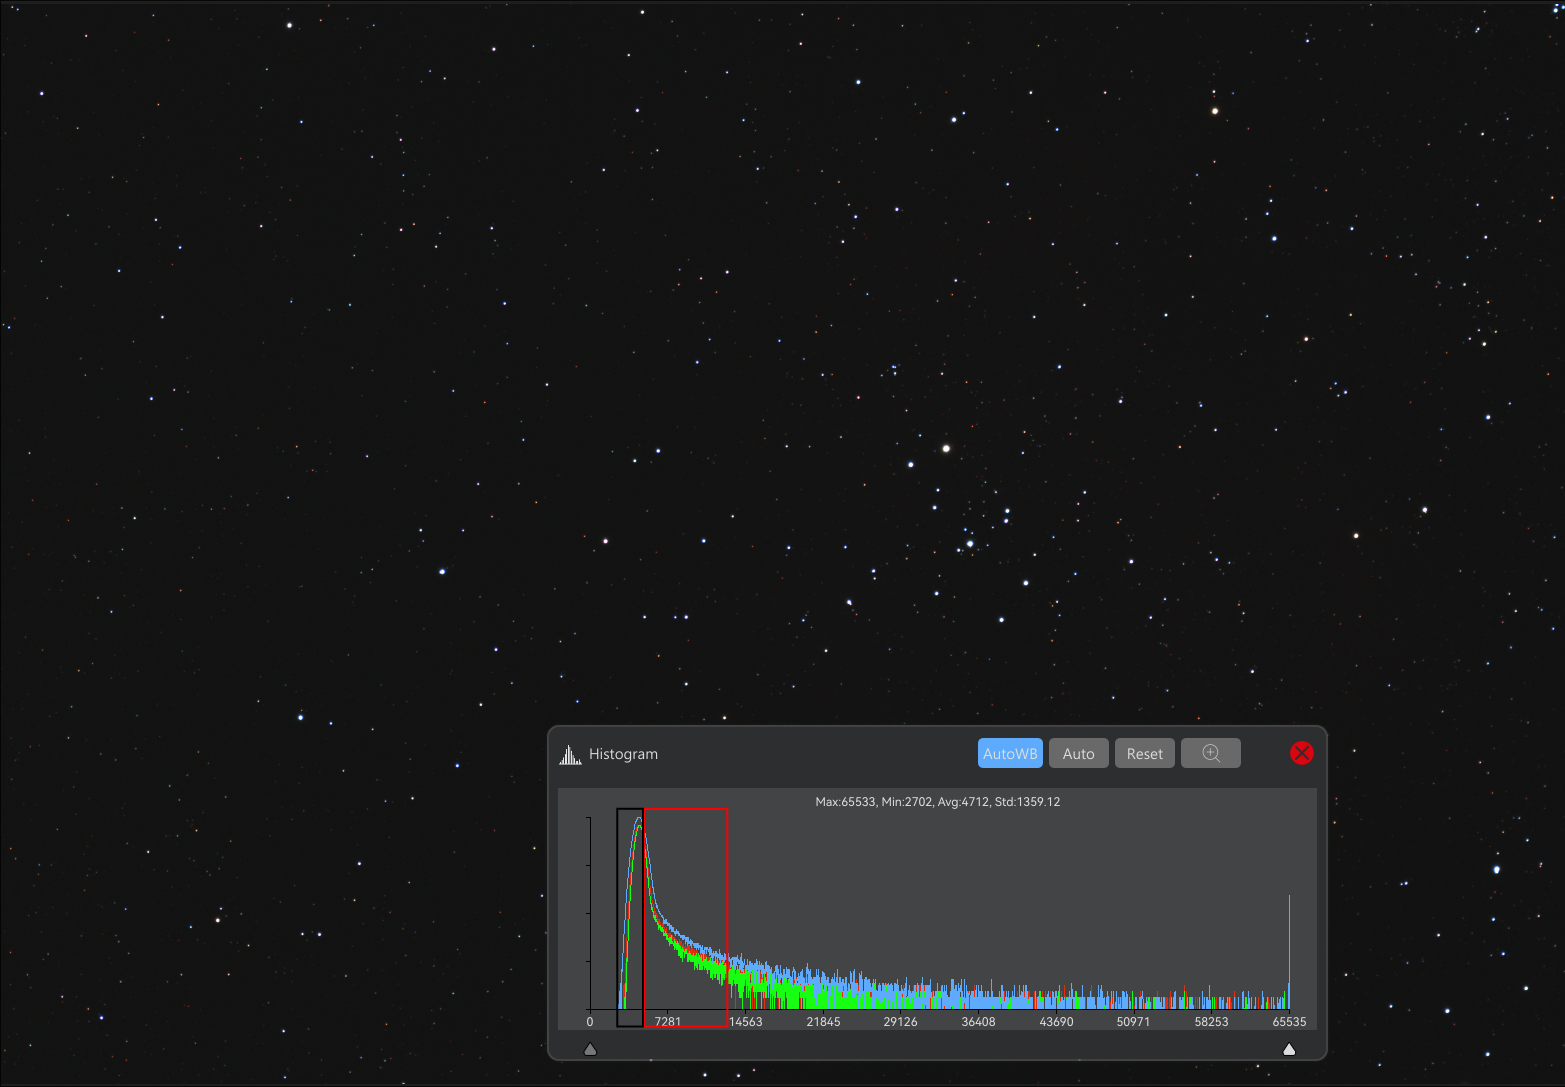
\includegraphics[width=0.78\textwidth]{assets/histogram.png} 
    \caption{Zobrazení histogramu před nelineární transformací} 
    \label{fig:histogram} 
\end{figure}

Z důvodu úspory výpočetního času systém neanalyzuje miliony pixelů každého snímku, ale provádí statistické vzorkování (analýzu každého stého pixelu). Z tohoto vzorku se vypočítává robustní mediánová absolutní odchylka (\ac{MAD}), která slouží k přesnému odhadu šumu pozadí bez zkreslení jasnými hvězdami. Následně se stanovují ořezové body pro nelineární roztažení histogramu. Systém podporuje režim propojených barevných kanálů pro zachování barevné věrnosti i režim nezávislých kanálů, který automaticky eliminuje silné barevné závoje způsobené světelným znečištěním.

\section{Hardwarová akcelerace vykreslování}
Opakovaný přepočet nelineárního strečinku na úrovni \acs{CPU} při každé změně parametrů nebo při rychlém přepínání snímků by vedl k neakceptovatelným latencím rozhraní. Výpočetní jádro proto surová data pouze normalizuje a předává je do prezentační vrstvy ve formě čistých textur. Výsledný efekt této transformace a okamžitého zobrazení skrytých detailů v uživatelském rozhraní je znázorněn na Obrázku~\ref{fig:autostf_preview}.

\begin{figure}[h]
    \centering
    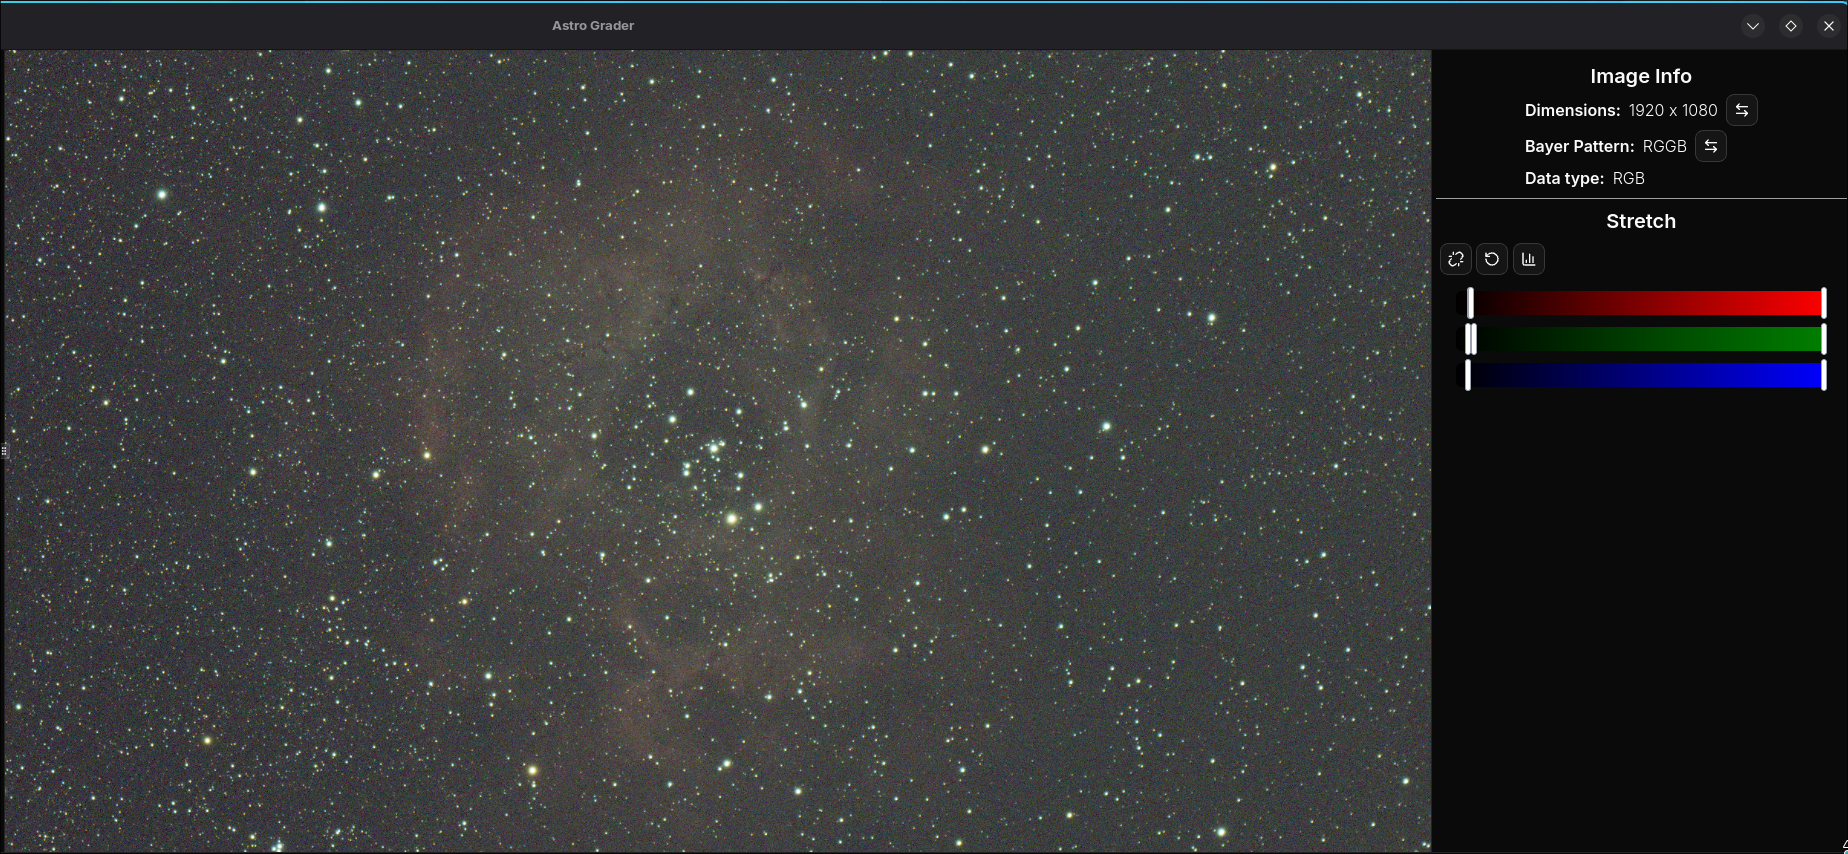
\includegraphics[width=0.78\textwidth]{assets/stretched.png}
    \caption{Vizualizace astronomického snímku po aplikaci automatické nelineární transformace jasu (AutoSTF).}
    \label{fig:autostf_preview}
\end{figure}

Vlastní nelineární transformace jasu a mapování histogramu probíhá v reálném čase přímo na grafické kartě počítače. K tomuto účelu se využívají vlastní \ac{WebGL} fragment shadery. Výpočetní zátěž se tím přenáší z procesoru na vysoce paralelní architekturu GPU, což umožňuje naprosto plynulé procházení a renderování snímků s nulovou latencí uživatelského rozhraní.
\chapter{Implementační architektura a algoritmy hodnocení kvality}
\label{ch:grading}

Tato kapitola se zabývá rozhodovací logikou hodnotícího systému, který plně automatizuje proces třídění a vyřazování expozic. Architektura podsystému kombinuje exaktní fyzikální limity s relativními statistickými modely, což umožňuje pružně reagovat na proměnlivé podmínky během akvizičních nocí.

\section{Režimy vyhodnocování (Globální vs. relační analýza)}
Systém nabízí dva konfigurovatelné režimy pro relativní porovnávání snímků, které zásadně ovlivňují chování statistického modelu a výpočet distribucí:

\begin{enumerate}
    \item \textbf{Lokální režim (po skupinách):} Statistické distribuce a mezní hodnoty se konstruují nezávisle pro každou pozorování relaci (noc). Tento přístup je vysoce inertní vůči dlouhodobým změnám atmosférických podmínek a je ideální pro izolované zpracování dat, kde kvalita z jedné noci nesmí ovlivnit přísnost klasifikace noci druhé.
    \item \textbf{Globální režim (křížový):} Výpočet normálního rozdělení a směrodatných odchylek probíhá napříč celým importovaným datasetem bez ohledu na datum pořízení. Tento režim nachází uplatnění při dlouhodobých projektech (tzv. \textit{multi-night projekty}), kdy je žádoucí vyřadit všechny snímky podprůměrné kvality vzhledem k celkovému historickému standardu dané optické soustavy.
\end{enumerate}

\section{Dvouprůchodový matematický hodnotící model}
Vlastní analýza kvality probíhá sekvenčně ve dvou oddělených průchodech. V prvním průchodu se provádí extrakce absolutních geometrických a kontrastních charakteristik z každé obrazové matice (počet hvězd, index \ac{HFD}, excentricita a kontrast pozadí). Z těchto normalizovaných hodnot se pomocí lineární kombinace s pevně stanovenými penalizačními vahami vypočítává surové skóre kvality. Použité konstanty a matematické limity pro výpočet surového skóre jsou uvedeny v Tabulce~\ref{tab:constants}.

\begin{table}[htbp]
    \centering
    \small
    \begin{tabular}{lllc}
        \hline
        \textbf{Metrika} & \textbf{Váhová konstanta ($W$)} & \textbf{Saturační limit pro optimum} & \textbf{Maximální penalizace} \\ \hline
        Počet hvězd & $W_{\text{star}} = 1.0$ & $5000$ hvězd & $0$ hvězd \\
        Profil \ac{FWHM} & $W_{\text{fwhm}} = 1.0$ & $\le 1.5$ px & $\ge 6.0$ px \\
        Kontrast pozadí & $W_{\text{bg}} = 1.5$ & \textit{Minimální \ac{RMS}} & $\text{Kontrast} \ge 10.0$ \\
        Excentricita & $W_{\text{ecc}} = 0.6$ & $0.0$ (dokonalá kružnice) & $\ge 0.6$ \\
        Profil stopy (\textit{Trail}) & $W_{\text{trail}} = 2.0$ & Bez lineárních prvků & Detekován průtah \\ \hline
    \end{tabular}
    \caption{Přehled interních konstant, vah a matematických limitů.}
    \label{tab:constants}
\end{table}

Ve druhém průchodu dochází k transformaci surového bodování na relativní skóre v rozsahu $\langle 0.0, 1.0 \rangle$ pomocí konstrukce lokální nebo globální Gaussovy distribuční křivky. Pozice snímku v této statistické distribuci určuje jeho finální zařazení metodou tří směrodatných odchylek ($3\sigma$).

Kromě automatické kategorizace systém implementuje sekundární hodnotící vrstvu, která dává uživateli plnou kontrolu nad výslednou přísností selekce. Prostřednictvím konfiguračního rozhraní (viz Obrázek \ref{fig:thresholding}) lze dynamicky měnit spodní hranici akceptovatelnosti (\textit{rejection threshold}). Změna tohoto parametru okamžitě spustí znovu výpočet metrik a zajistí znovu klasifikaci snímků do správných kategorií na základě nové hranice akceptovatelnosti.

\begin{figure}[htbp]
    \centering
    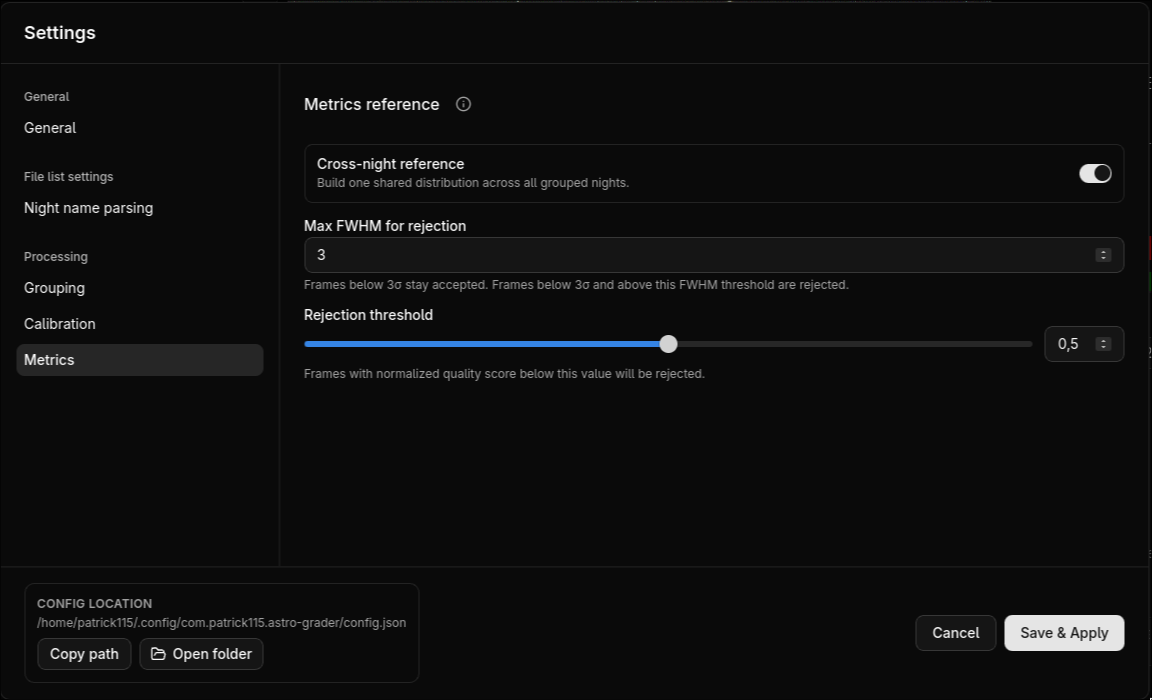
\includegraphics[width=0.60\textwidth]{assets/treshold_settings.png}
    \caption{Konfigurační panel uživatelského rozhraní pro dynamické nastavení prahových hodnot a spodní hranice akceptovatelnosti relativního skóre.}
    \label{fig:thresholding}
\end{figure}

\section{Ochranná logika a deterministické pojistky}
Aby se zabránilo selhání relativního statistického modelu v anomálních situacích (například pokud jsou vlivem souvislé oblačnosti znehodnoceny všechny snímky z dané noci, což by u čistě relativního modelu vedlo k chybnému schválení nejméně poškozených expozic), systém obsahuje autonomní ochranné pojistky.

Snímek je okamžitě klasifikován stavem vyřazení s příslušným chybovým hlášením bez ohledu na svou pozici v normálním rozdělení, pokud nastane jedno z následujících kritérií:
\begin{itemize}
    \item Celkový počet detekovaných bodových zdrojů klesne pod kritickou mez, což indikuje přítomnost husté oblačnosti nebo technické selhání expozice.
    \item Průměrná excentricita profilů hvězd překročí pevný práh $0.6$, což detekuje závažné mechanické chyby v pointaci montáže nebo přítomnost výrazných stop družic a meteorů (\textit{star trails}).
    \item Globální kontrast pozadí překročí absolutní kritickou hodnotu $15.0$ vlivem extrémního rozptylu světla na vysoké oblačnosti či při náhlém osvícení měsícem.
\end{itemize}

Všechny tyto metriky jsou zobrazeny v \ac{UI} a dovolují jednoduše uživateli vybrat zamítnuté (rejected) snímky a buď provést jejich smazání, nebo je přesunout do jiné složky (viz Obrázek \ref{fig:metrics_list}).

\begin{figure}[htbp]
    \centering
    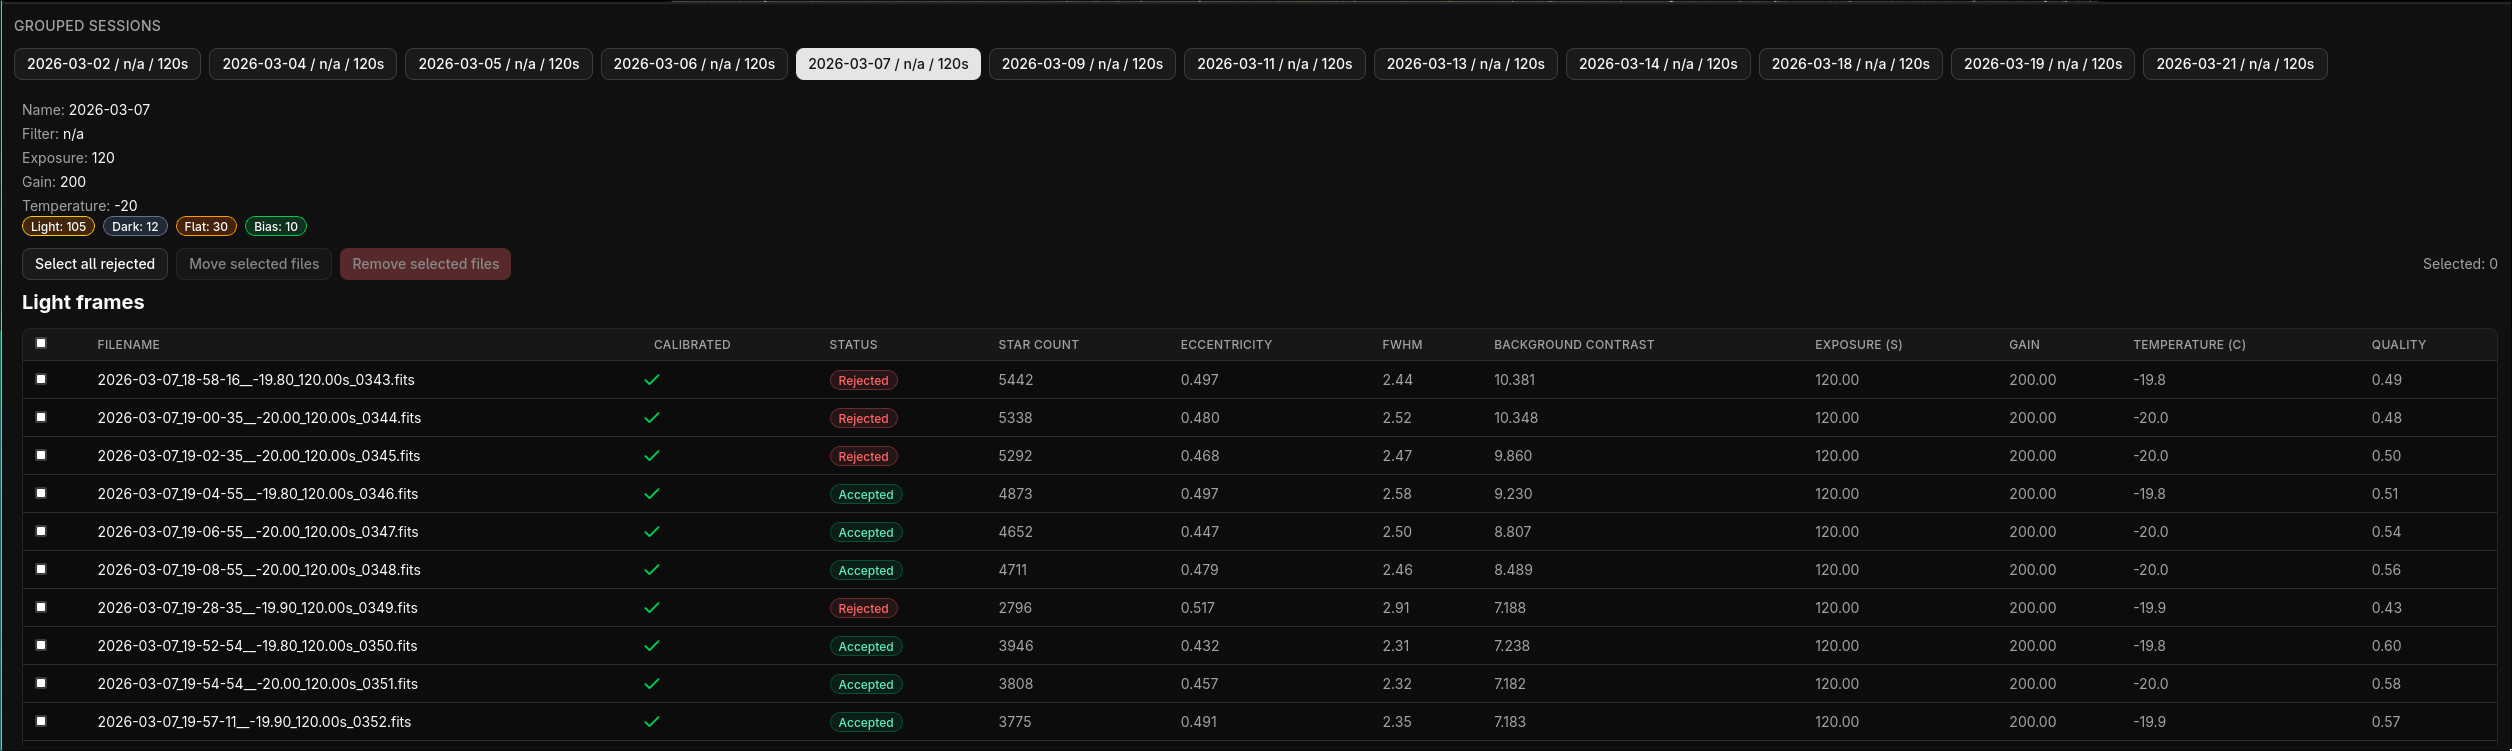
\includegraphics[width=0.85\textwidth]{assets/table.png}
    \caption{Ukázka vygenerovaného seznamu analyzovaných souborů v uživatelském rozhraní se zobrazením vypočtených fyzikálních metrik a finálního stavu.}
    \label{fig:metrics_list}
\end{figure}
\chapter{Závěr}
\label{ch:zaver}

V rámci tohoto semestrálního projektu byla úspěšně navržena a implementována kompletní analytická a deterministická část systému pro automatizované předběžné zpracování astronomických snímků. Systém úspěšně integruje nízkoúrovňové operace pro čtení datových struktur \ac{FITS}, automatizovaný modul pro segmentaci kalibračních dat a matematické subsystémy pro mřížkový odhad pozadí a profilování geometrie hvězd. Spojení vysokovýkonného výpočetního jádra a lehkého reaktivního klientského rozhraní prokázalo vysokou propustnost dat při matematických transformacích pixelů, přičemž celkový přehled o architektuře hotového uživatelského rozhraní je znázorněn na Obrázku~\ref{fig:full_ui_screenshot}.

\begin{figure}[htbp]
    \centering
    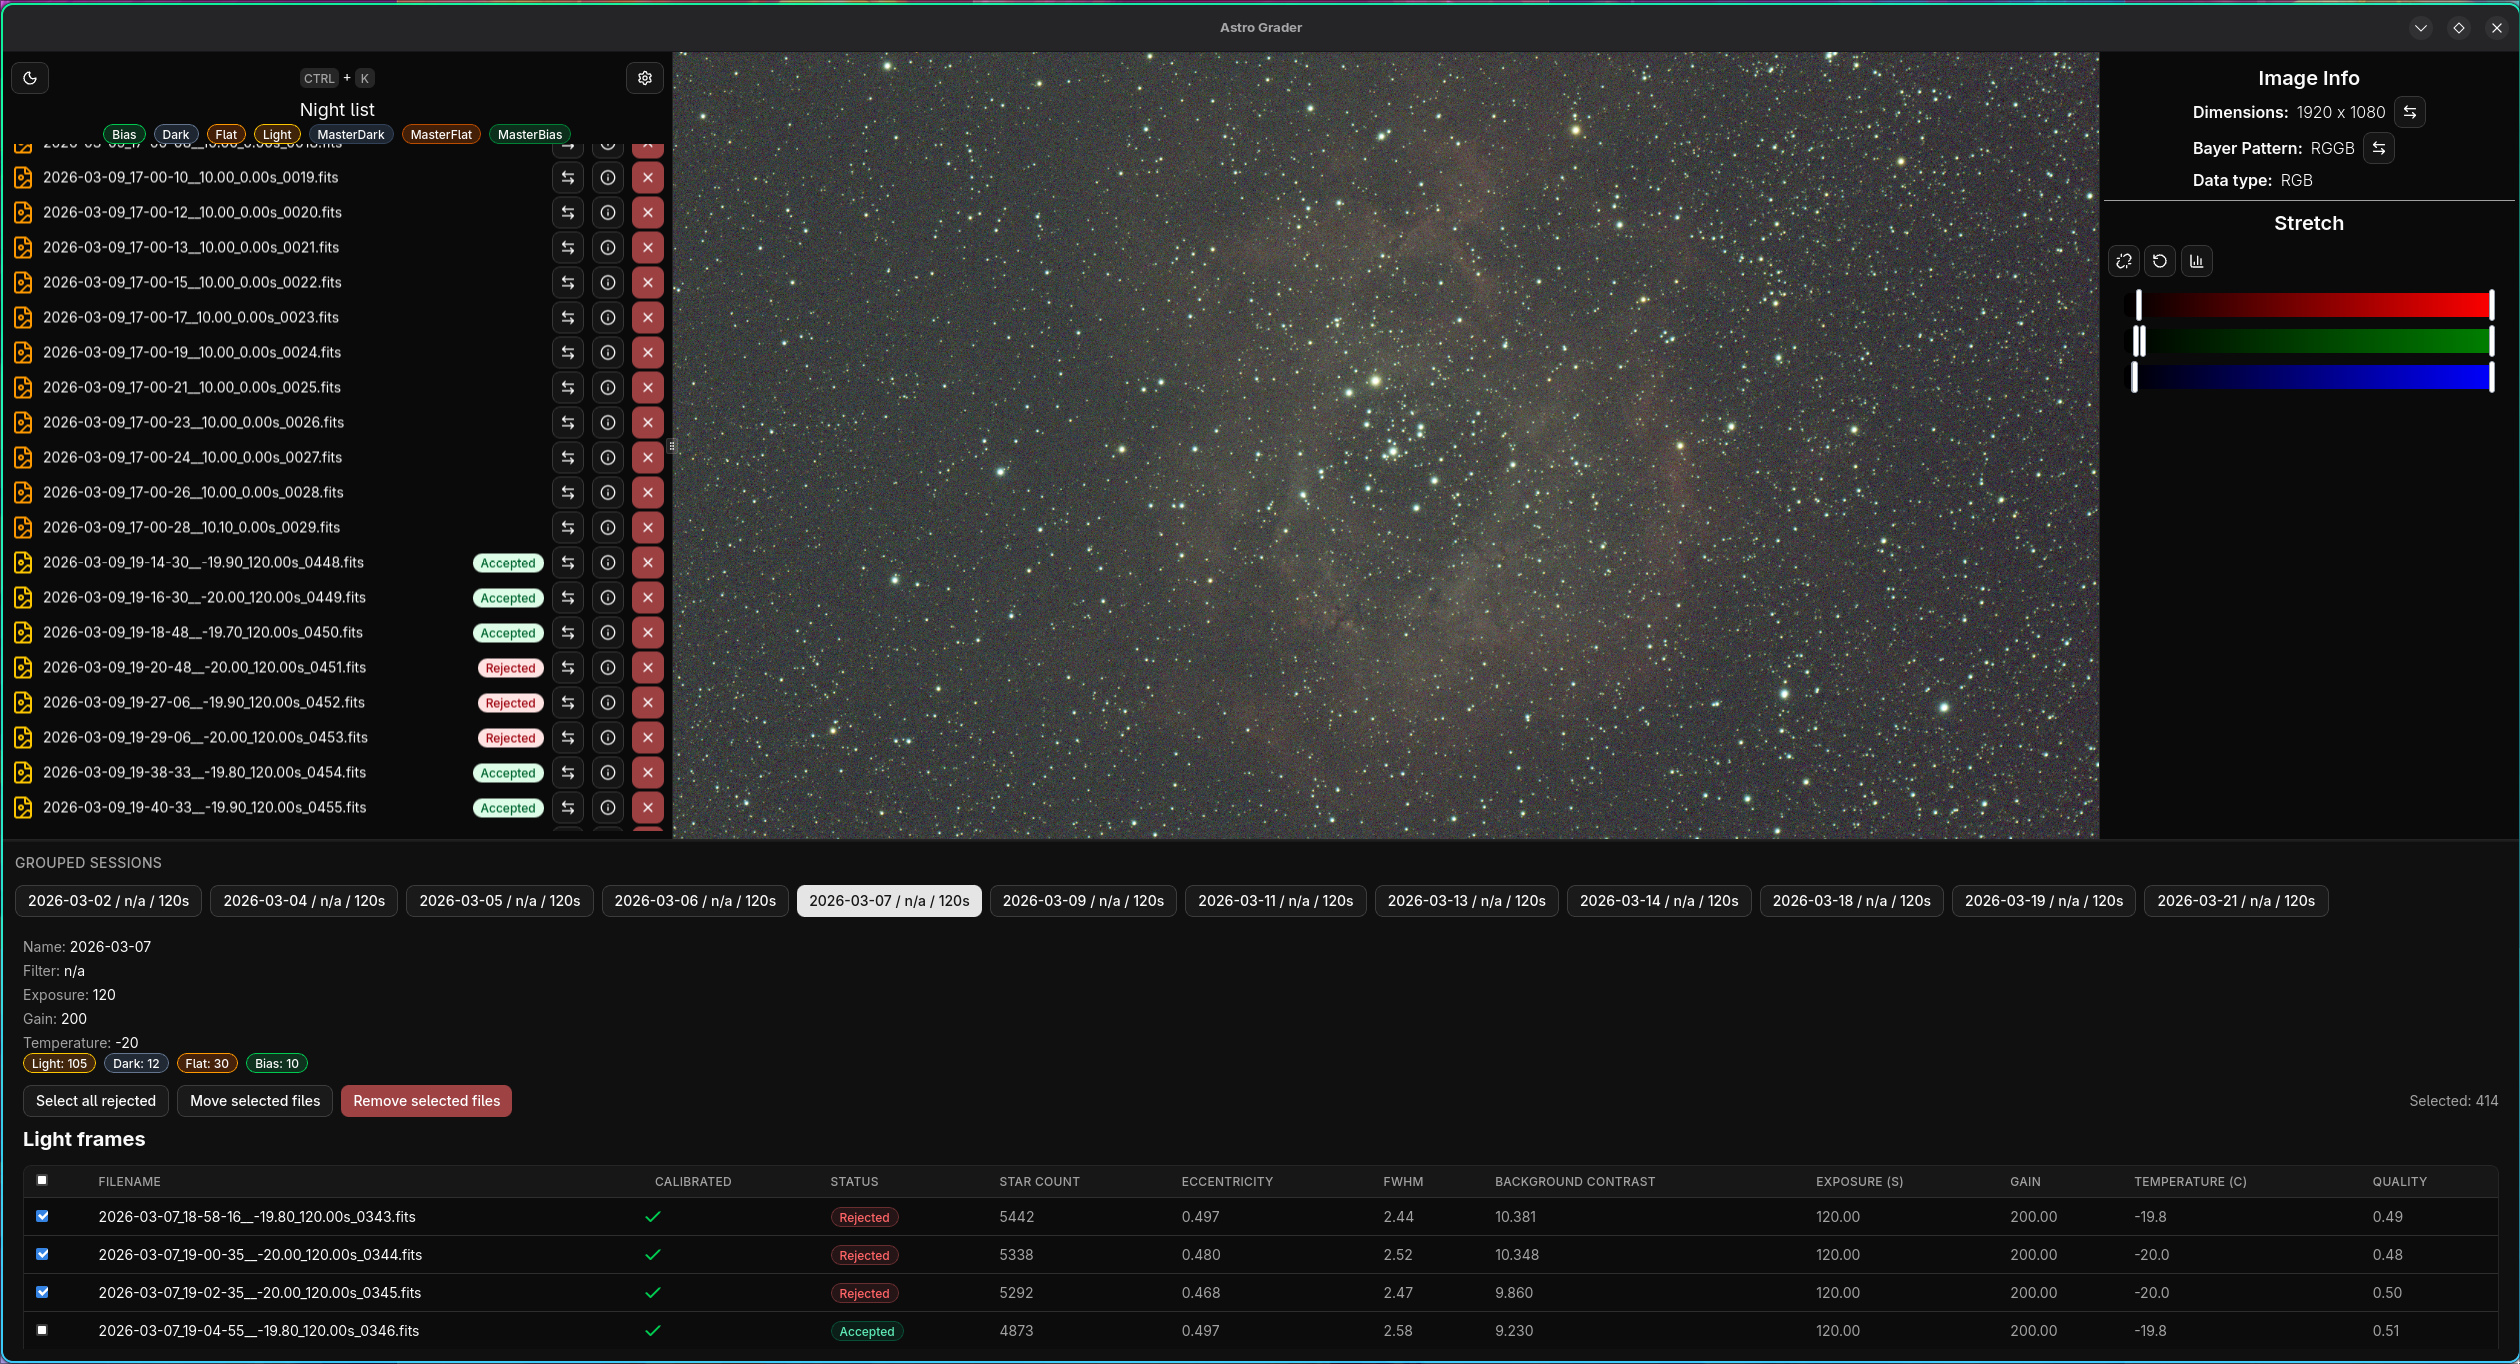
\includegraphics[width=0.95\textwidth]{assets/full_overview.png}
    \caption{Kompletní grafické uživatelské rozhraní vyvinuté aplikace.}
    \label{fig:full_ui_screenshot}
\end{figure}

\section{Výkonnostní analýza a limity diskových operací}
Pro exaktní ověření propustnosti systému byl v rámci testování využit reálný astrofotografický dataset emisní mlhoviny Rozeta (\textit{Caldwell 49 / NGC 2244}) čítající celkem 1104 surových snímků. Testovací proces zahrnoval kompletní kalibrační řetězec, tedy matematické sloučení desítek dílčích snímků plochého pole (\textit{Flat}), temných snímků (\textit{Dark}) i ofsetů (\textit{Bias}) do příslušných referenčních předloh, následnou aplikaci pixelové aritmetiky na snímky a finální extrakci profilových metrik.


Celkový čas zpracování této sady činil 32 minut. Z podrobné profilace výpočetního času vyplynulo, že samotná kalibrační fáze zabrala 30 minut, což představuje majoritní režii celé pipeline. Přestože matematické výpočty nad maticemi pixelů probíhají masivně paralelně, výpočetní vlákna jsou zásadně limitována synchronním charakterem diskových operací. V současné implementaci totiž každé vlákno v rámci své rutiny sekvenčně provádí načtení surového souboru z disku, jeho kalibraci v paměti a okamžitý zápis výsledku zpět na trvalé úložiště. Procesorový čas je tak degradován čekáním na dokončení I/O operací diskového subsystému.

Jako budoucí optimalizační krok se proto jeví restrukturalizace kalibračního modulu do architektury typu producent-konzument (\textit{Producer-Consumer}). Tento model předpokládá vyčlenění dedikovaných asynchronních vláken určených výhradně pro sekvenční čtení surových dat do sdílené paměťové fronty a paralelní zápis hotových souborů z výstupní fronty na disk. Výpočetní jádra by tak byla kontinuálně saturována čistě matematickými transformacemi pixelů bez blokování I/O operacemi, což by dramaticky zkrátilo celkovou časovou náročnost u extrémně rozsáhlých datových sad.

\section{Kritické vyhodnocení úspěšnosti hodnotících algoritmů}
Z hlediska detekce fatálních geometrických a atmosférických vad v obrazových datech vykazuje navržený deterministický aparát vysokou míru spolehlivosti. Snímky, které jsou znehodnoceny úplným zacloněním oblačností (vedoucím k poklesu počtu detekovaných hvězd pod kritickou mez) nebo závažnými chybami v chodu montáže (projevujícími se protažením profilů hvězd do stop), jsou systémem spolehlivě identifikovány a automaticky vyřazovány.

Limitace lineární kombinace skalárních statistik se však projevují při specifických atmosférických jevech, jako je přechod nízké, poloprůhledné oblačnosti či vysokého závoje. V těchto situacích dochází k dramatickému útlumu difuzního světla z hlubokého vesmíru, což vede k téměř kompletní ztrátě slabých struktur emisních mlhovin v mezihvězdném pozadí. Bodové zdroje s vysokým vlastním jasem (hvězdy) však přesto dokážou touto vrstvou prostoupit s dostatečným odstupem signálu od šumu, což segmentačnímu algoritmu stále umožňuje jejich úspěšnou extrakci. 

V důsledku matematické zranitelnosti implementovaného modelu výpočtu kontrastu pozadí, který v těchto hraničních stavech nedokáže dostatečně penalizovat plošnou ztrátu transparentnosti mikrokontrastu mlhoviny, systém takto degradované snímky chybně klasifikuje jako vyhovující a propouští je do dalšího zpracování.

Tento jev jasně ilustruje Obrázek~\ref{fig:score_comparison}. Při srovnání dvou expozic se shodně vypočteným relativním skóre $0.5$ je patrné, že pevně stanovené váhové koeficienty nedokážou flexibilně kompenzovat vzájemnou korelaci mezi jasem pozadí a lokální transparentností. Jeden ze snímků vykazuje optimální strukturální data, zatímco druhý je pro finální skládání vědeckých dat nepoužitelný. Nutnost neustálého manuálního ladění (\textit{tweakingu}) prahových hodnot pro různé typy oblohy a snímačů potvrzuje limity čistě matematického modelování a tvoří klíčový argument pro přechod k metodologické fázi hlubokého učení.

\begin{figure}[htbp]
    \centering
    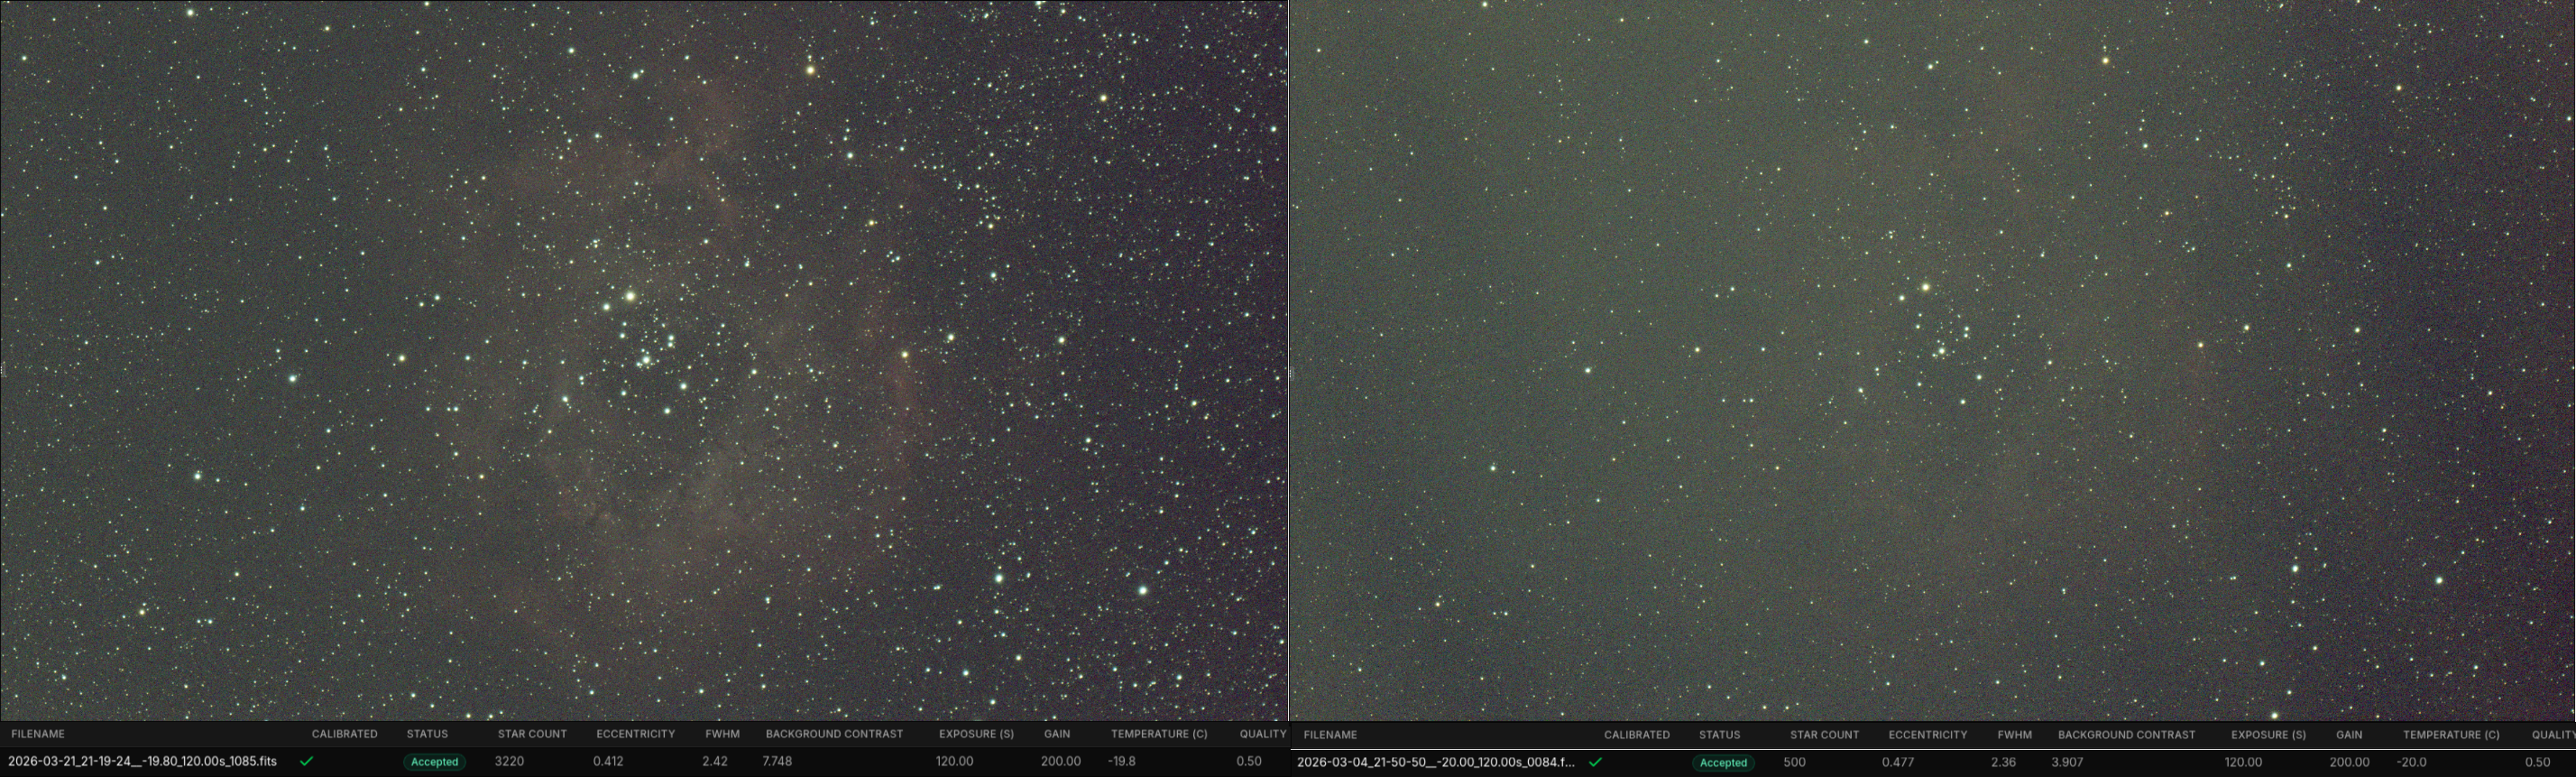
\includegraphics[width=1.0\textwidth]{assets/score_comparison.png}
    \caption{Srovnání dvou expozic se shodným vypočteným skóre (0.5)}
    \label{fig:score_comparison}
\end{figure}

Navzdory těmto drobným limitacím v hraničních oblastech systém jako celek funguje stabilně a poskytuje objektivní, reprodukovatelná data. Po mírné dodatečné korekci vah je systém plně připraven plnit svou primární roli, kterou je rychlé generování autoritativních anotačních štítků pro přípravu tréninkových dat.

\section{Návaznost na diplomovou práci a integrace neuronových sítí}
Zjištěná závislost deterministického přístupu na empirickém ladění prahových hodnot tvoří logický most k navazující diplomové práci. Cílem druhé fáze projektu bude kompletní nahrazení stávajícího statistického rozhodovacího bloku vlastním modelem hlubokého učení. 

Dokončená desktopová aplikace bude v této nadcházející etapě využita jako expertní anotační prostředí. Uživatelsky schválené, revidované a vyřazené snímky z testovacích relací poslouží jako validovaná tréninková množina. Vývojový plán předpokládá integraci tréninkového rozhraní přímo do klientské vrstvy SvelteKitu. To umožní koncovému uživateli provádět lokální jemné doladění (\textit{fine-tuning}) lehké konvoluční neuronové sítě (\ac{CNN}) přímo na specifické optické vady, vinětaci a fixní šumové charakteristiky jeho konkrétní hardwarové sestavy, čímž se zcela odstraní nutnost jakéhokoliv manuálního nastavování matematických limitů.

% =========================================================================
% LITERATURA A CITACE (Bibliography)
% =========================================================================
\clearpage
\printbibliography[title={Literatura}, heading=bibintoc]

\end{document}